\chapter{Diseño de la solución propuesta para la automatización de la rotación de circuitos eléctricos}

\section{Introducción}

El presente capítulo tiene como objetivo describir y fundamentar el diseño de la solución informática propuesta para resolver el problema científico identificado en el capítulo anterior, relacionado con las limitaciones del proceso manual de rotación de circuitos eléctricos ante déficit de generación en el Despacho Provincial de Carga. En correspondencia con los fundamentos teóricos, regulatorios y metodológicos previamente sistematizados, este capítulo expone la concepción arquitectónica, los artefactos de requisitos, las tecnologías seleccionadas y la descripción funcional de la plataforma web desarrollada \cite{pressman2020}.

El diseño de la solución se enmarca en los principios de la Ingeniería de Software orientada a sistemas de misión crítica, donde la arquitectura constituye un elemento determinante para garantizar calidad, mantenibilidad y desempeño \cite{bass2013}. En entornos energéticos regulados, el diseño no puede limitarse a la implementación funcional, sino que debe asegurar coherencia estructural, separación de responsabilidades y cumplimiento de requisitos operativos de alta disponibilidad \cite{gomez2016}. Por tanto, la solución propuesta fue concebida bajo una arquitectura desacoplada cliente-servidor, basada en Next.js para el frontend, NestJS para el backend y SQL Server 2008 como sistema de persistencia legacy.

El capítulo se organiza en tres secciones principales: (1) fundamentos tecnológicos para el desarrollo del sistema; (2) descripción de la solución propuesta; y (3) ingeniería de requisitos del sistema.

% ------------------------------------------------------------------
\section{Fundamentos Tecnológicos para el Desarrollo del Sistema}

La selección de las tecnologías se fundamentó en tres criterios principales: la necesidad de una arquitectura cliente-servidor para accesibilidad multiusuario, la compatibilidad con la infraestructura de datos legacy en el Despacho Provincial de Carga~\citep{villalba2021}, y la adecuación a los requerimientos operativos de alta disponibilidad del Despacho Nacional de Carga (DNC)~\citep{union2023}.

\subsection{Capa de presentación: Next.js y React}
Para el desarrollo de la capa de presentación se seleccionó el framework \textbf{Next.js} basado en la biblioteca \textbf{React}. Esta decisión permitió el desarrollo de una \textit{Single Page Application} (SPA) que garantiza una interfaz de usuario fluida y reactiva. El uso de \textbf{Tailwind CSS} para el estilizado facilitó la creación de componentes visuales de alto rendimiento, optimizados para la visualización de grandes volúmenes de datos operativos. A diferencia de las aplicaciones de escritorio tradicionales, esta tecnología permite el acceso al sistema desde cualquier nodo de la red local sin necesidad de instalaciones locales.

\subsection{Capa de servicios: NestJS}
Para la capa de servicios se implementó \textbf{NestJS}, un framework de Node.js progresivo que permite construir aplicaciones del lado del servidor eficientes y escalables. NestJS actúa como una API REST robusta que centraliza la lógica de negocio y el algoritmo de rotación. Esta capa gestiona la comunicación con los servidores \textbf{SQL Server 2008} mediante una capa de abstracción de datos, ejecutando consultas optimizadas a las bases SIGERE y PSFV~\citep{jones2019}. El backend garantiza que el procesamiento del déficit y la priorización de circuitos ocurran en un entorno controlado, devolviendo al cliente únicamente la información procesada y validada.

\subsection{Persistencia: SQL Server 2008 (consideraciones y limitaciones)}
La gestión de persistencia de datos se mantuvo en SQL Server 2008, dado que constituía la infraestructura ya establecida y validada en el Despacho Provincial~\citep{ministerio2023}. El sistema aprovechó procedimientos almacenados existentes y garantizó la integridad transaccional necesaria para operaciones de maniobra eléctrica.

\textbf{Nota sobre la versión:} SQL Server 2008 es una versión cuyo soporte extendido finalizó en 2019. Su uso en el proyecto responde a que la infraestructura del Despacho no ha sido migrada por restricciones presupuestarias y organizativas. Esta limitación se asume como un riesgo controlado: la comunicación entre NestJS y la base de datos se realiza únicamente mediante consultas parametrizadas y procedimientos almacenados, sin exponer la base directamente a la red. No obstante, se recomienda en futuras versiones migrar a SQL Server 2019 o PostgreSQL para garantizar seguridad y soporte a largo plazo.

La integración entre el backend moderno y la base de datos heredada se realizó mediante conectores optimizados que aseguran tiempos de respuesta inferiores a los 3 segundos, cumpliendo con estándares internacionales para sistemas de automatización energética~\citep{ansi2018}.

\subsection{Metodología de desarrollo}
Para la metodología de desarrollo se adoptó la Programación Extrema (XP) como marco ágil de trabajo~\citep{beck2000}. Esta elección permitió organizar el desarrollo en iteraciones cortas (una o dos semanas), donde al final de cada iteración se entregaba un incremento funcional validado directamente por los especialistas del Despacho. La retroalimentación continua del cliente facilitó la adaptación del sistema a las necesidades emergentes del flujo de trabajo real.

% ------------------------------------------------------------------
\section{Descripción de la Solución Propuesta}

La plataforma web automatizada integra y procesa información dispersa en múltiples fuentes~\citep{villalba2021}, generando órdenes optimizadas de rotación de circuitos ante déficit de generación~\citep{gomez2016}.

\begin{figure}[htbp]
\centering
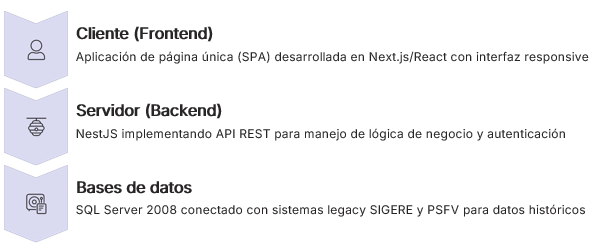
\includegraphics[width=0.82\textwidth]{img/arquitectura_sistema.png}
\caption{Arquitectura del sistema automatizado de rotación de circuitos (Next.js - NestJS)}
\label{fig:arquitectura_sistema}
\end{figure}

Como se ilustra en la Figura~\ref{fig:arquitectura_sistema}, el sistema implementa una \textbf{arquitectura desacoplada} que organiza los componentes en dos bloques fundamentales: un cliente web reactivo y un servidor de aplicaciones.

\subsection{Capa de Presentación (Frontend: Next.js/React)}
La interfaz de usuario se desarrolló como una SPA utilizando \textbf{React y Tailwind CSS}~\citep{pressman2020}. Permite visualizar el déficit en tiempo real mediante componentes reactivos, supervisar propuestas automatizadas en tablas dinámicas y gestionar excepciones operativas (circuitos asegurados). El estado global se gestiona mediante \textbf{Context API}, asegurando sincronización de datos entre vistas sin recargar la página.

\subsection{Capa de Lógica de Negocio (Backend: NestJS)}
El núcleo algorítmico reside en el servidor con \textbf{NestJS}. Implementa el cálculo automatizado del déficit:
\[
\text{Déficit} = \sum \text{MW\_Afectados} - \sum \text{MW\_Asegurados}
\]

\begin{center}
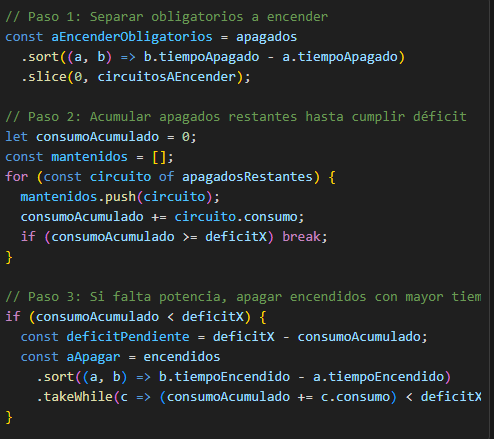
\includegraphics[width=0.8\textwidth]{img/algoritmo_rotacion_min.png}
\captionof{figure}{Algoritmo minimalista de rotación de circuitos}
\label{fig:algoritmo-rotacion}
\end{center}

El backend aplica algoritmos de priorización inteligente, excluyendo automáticamente circuitos críticos o bajo mantenimiento, y expone una \textbf{API REST} que procesa solicitudes del cliente, eliminando la carga de cálculo en el navegador~\citep{zhou2023}.

\subsection{Capa de Acceso a Datos (Persistencia)}
El sistema establece una conexión optimizada con \textbf{SQL Server 2008} (SIGERE y PSFV)~\citep{jones2019}. El backend actúa como orquestador, unificando tablas críticas como \texttt{MSW\_Aseguramientos} y \texttt{ap\_curvas}, resolviendo la fragmentación histórica de los datos~\citep{ministerio2023}.

\subsection{Flujo de Operación del Sistema}
El proceso sigue esta secuencia:
\begin{enumerate}
    \item El operador introduce parámetros en la interfaz de React.
    \item El cliente envía una petición asíncrona mediante \textbf{Axios} al servidor NestJS.
    \item El servidor consulta las bases SQL Server mediante procedimientos almacenados.
    \item El motor de lógica aplica los algoritmos de priorización.
    \item La respuesta se envía al cliente en formato JSON.
    \item La interfaz se actualiza instantáneamente reflejando la propuesta de rotación.
\end{enumerate}

\subsection{Integración y Seguridad}
La solución se integra con la infraestructura existente mediante compatibilidad total con SQL Server 2008, seguridad con \textbf{JWT} para control de acceso y rendimiento optimizado (cálculo en menos de 3 segundos). Al ser una aplicación web, garantiza interoperabilidad desde cualquier dispositivo con navegador dentro de la red del Despacho.

\subsection{Ventajas de la Arquitectura Web}
Esta arquitectura ofrece:
\begin{itemize}
    \item \textbf{Escalabilidad}: permite añadir funcionalidades sin afectar al cliente.
    \item \textbf{Despliegue centralizado}: elimina la necesidad de instalar software en cada terminal.
    \item \textbf{Mantenibilidad}: separa claramente la UI de la lógica de datos.
\end{itemize}
La solución reduce el tiempo de respuesta de 45 minutos a segundos, elimina errores manuales y aprovecha plenamente los datos legacy.

% ------------------------------------------------------------------
\section{Ingeniería de Requisitos del Sistema}

La identificación de necesidades se realizó mediante un proceso estructurado de levantamiento con especialistas operativos del Despacho Provincial de Carga~\citep{union2023}. El objetivo era reducir el tiempo de respuesta operativo a menos de 5 minutos mediante una interfaz reactiva y precisa~\citep{pressman2020}. \textbf{Nota:} Durante la implementación se superó este objetivo, alcanzando tiempos de 2 a 3 segundos, como se reporta en el Capítulo III.

\subsection{Objetivos de rendimiento}
La Tabla~\ref{tab:objetivos_rendimiento} sintetiza los objetivos de rendimiento derivados del análisis de brechas.

\begin{table}[H]
\centering
\caption{Objetivos de rendimiento del sistema automatizado}
\label{tab:objetivos_rendimiento}
\begin{tabular}{|l|c|c|}
\hline
\textbf{Parámetro} & \textbf{Estado Actual} & \textbf{Objetivo} \\ \hline
Tiempo de respuesta & 30--45 minutos & $<$ 5 minutos (superado a 2-3 s) \\ \hline
Precisión en cálculos & 90--95\% & 100\% \\ \hline
Consistencia operativa & Baja (Manual) & Alta (Algorítmica) \\ \hline
Capacidad de simulación & Nula & Completa (Escenarios) \\ \hline
Disponibilidad de datos & Dispersa & Centralizada (API) \\ \hline
\end{tabular}
\end{table}

\subsection{Requisitos funcionales y su organización en historias de usuario}
Se identificaron 45 funcionalidades, que se agruparon en 11 historias de usuario (ver Anexo A). La Tabla~\ref{tab:hu_coverage} muestra la correspondencia entre módulos y las historias que los cubren.

\begin{table}[H]
\centering
\caption{Cobertura de funcionalidades por historias de usuario}
\label{tab:hu_coverage}
\begin{tabular}{|l|c|l|}
\hline
\textbf{Módulo} & \textbf{Número de funcionalidades} & \textbf{HU asociadas} \\ \hline
Seguridad y usuarios & 8 & HU1, HU2, HU3 \\ \hline
Gestión de circuitos y aseguramientos & 12 & HU4, HU5 \\ \hline
Rotación y algoritmos & 15 & HU6, HU7, HU8 \\ \hline
Reportes y monitoreo & 10 & HU9, HU10, HU11 \\ \hline
\end{tabular}
\end{table}

La documentación de requisitos siguió las prácticas de XP, con historias de usuario que describen cada funcionalidad desde la perspectiva del operador. A continuación se resumen los módulos:

\begin{itemize}
    \item \textbf{Módulo de Seguridad y Usuarios}: acceso restringido con credenciales, gestión de roles (Administrador/Operador), sesión segura mediante JWT. Cubierto por HU1, HU2, HU3.
    \item \textbf{Módulo de Gestión de Circuitos y Aseguramientos}: sincronización con SIGERE y PSFV, clasificación automática de circuitos, gestión de circuitos críticos ("asegurados"). Cubierto por HU4, HU5.
    \item \textbf{Módulo de Rotación y Algoritmos}: cálculo automático del déficit, generación de propuestas por prioridad de bloques, validación de restricciones del DNC, ajustes manuales. Cubierto por HU6, HU7, HU8.
    \item \textbf{Módulo de Reportes y Monitoreo}: exportación de órdenes a PDF/Excel, dashboard interactivo con alertas visuales y estadísticas históricas. Cubierto por HU9, HU10, HU11.
\end{itemize}

\subsection{Requisitos no funcionales}
La Tabla~\ref{tab:requisitos_no_funcionales} resume los requisitos no funcionales que garantizan calidad y sostenibilidad.

\begin{table}[H]
\centering
\caption{Requisitos no funcionales del sistema (RNF)}
\label{tab:requisitos_no_funcionales}
\begin{tabular}{|l|l|}
\hline
\textbf{Categoría} & \textbf{Especificación} \\ \hline
Rendimiento & Tiempo de respuesta de la API $<$ 2 segundos \\ \hline
Seguridad & Autenticación mediante JWT (JSON Web Tokens) \\ \hline
Disponibilidad & Uptime del servicio $\geq$ 99.5\% \\ \hline
Usabilidad & Interfaz \textit{Responsive} (Tailwind CSS) \\ \hline
Interoperabilidad & Conexión con SQL Server 2008 legacy \\ \hline
Mantenibilidad & Arquitectura cliente-servidor desacoplada \\ \hline
Escalabilidad & Capacidad para gestionar 500+ circuitos en tiempo real \\ \hline
\end{tabular}
\end{table}

La transición a una arquitectura web permite cumplir con criterios de mantenibilidad y escalabilidad que los sistemas de escritorio no ofrecen~\citep{cujae2021}.

% ------------------------------------------------------------------
\section{Conclusiones del capítulo}

\begin{enumerate}
    \item La selección tecnológica basada en Next.js, NestJS y SQL Server 2008 respondió a los criterios de arquitectura cliente-servidor para accesibilidad multiusuario, compatibilidad con la infraestructura legacy existente y adecuación a los requerimientos de alta disponibilidad del DNC. Se discute explícitamente la obsolescencia de SQL Server 2008 como una limitación asumida, dejando abierta la recomendación de migración futura.
    
    \item La arquitectura desacoplada separa claramente la capa de presentación, la lógica de negocio y el acceso a datos, garantizando escalabilidad, mantenibilidad y despliegue centralizado. El flujo de operación definido reduce drásticamente los tiempos de respuesta y elimina errores humanos.
    
    \item La ingeniería de requisitos permitió formalizar 45 funcionalidades organizadas en cuatro módulos lógicos, documentadas mediante 11 historias de usuario. Los objetivos de rendimiento (respuesta <5 min) fueron superados (2-3 s), como se validará en el Capítulo III.
    
    \item La integración de los fundamentos tecnológicos, la descripción de la solución y la ingeniería de requisitos proporciona una base sólida para la implementación y validación de la plataforma, asegurando coherencia con el problema científico.
\end{enumerate}